The computer exercises parts of the practicals focus on working with MADX, the CERN software to simulate beam dynamics and optimize beam optics in particle accelerators.
\section{Part I - Building your own FODO lattice and tracking}
As shown in listing \ref{lst:FODOcell} in a first step a single FODO cell is defined. Between two quadrupoles is a drift space \textit{dr} of length $D$. The quadrupoles are thin-lens elements defined over the \textit{multipole} command. The focussing quadrupole \textit{qf} has a strength of $1/f$, while the defocussing one \textit{qd} has $-1/f$, with $f$ being the focal length.\\
These elements are combined into a FODO cell \textit{fodo1} and the whole ring consists only of this one cell.\\
The particles are set to be electrons at an energy of $1.3\mathrm{\,GeV}$.

\begin{lstlisting}[caption=Defining the FODO cell,label={lst:FODOcell}]
D=1;
f=1;
qf: multipole, knl={0, 1/f};
dr: drift, l=D;
qd: multipole, knl={0, -1/f};
fodo1: line=(qf, dr, qd,dr);
ring: line=(fodo1);

beam, particle=electron, energy=1.3, sequence=ring;
use, sequence=ring;
\end{lstlisting}

In order to calculate the trajectories element by element through the thin-lens elements the \textit{track} command is used. It takes a relative momentum offset for the reference closed orbit (\textit{deltap}). The initial trajectory coordinates are given per trajectory/particle with one \textit{start} command. Here there particle has no momentum offset but starts slightly off center, so that the effects of the FODO cell can be seen.
The the actual tracking is triggered (\textit{run}) for the number of \textit{turns} given.\\
The results of the coordinate calculations per turn are saved in a table and with the \textit{plot} command plotted as phase space ellipses ($px$ over $x$ and $py$ over $y$).

\begin{lstlisting}[caption=Tracking,label={lst:tracking}]
track,  onepass, dump, deltap=0.001;
        start, x=3e-3, px=0, y=3e-3, py=0;
        run, turns=100;
endtrack;
plot, table=track, haxis=x, vaxis=px, particle=1, colour=1000, multiple, symbol=3, file=turns100d1f1;
plot, table=track, haxis=y, vaxis=py, particle=1, colour=1000, multiple, symbol=3, file=turns100d1f1;
\end{lstlisting}

Figure \ref{fig:ellipse} shows the phase space ellipses of the one defined electron for $x$ and $y$ sub-spaces for $D=f=1\,\mathrm{m}$, which results in a stable motion.

\begin{figure}[tbp]
    \centering
    \begin{minipage}{0.49\textwidth}
        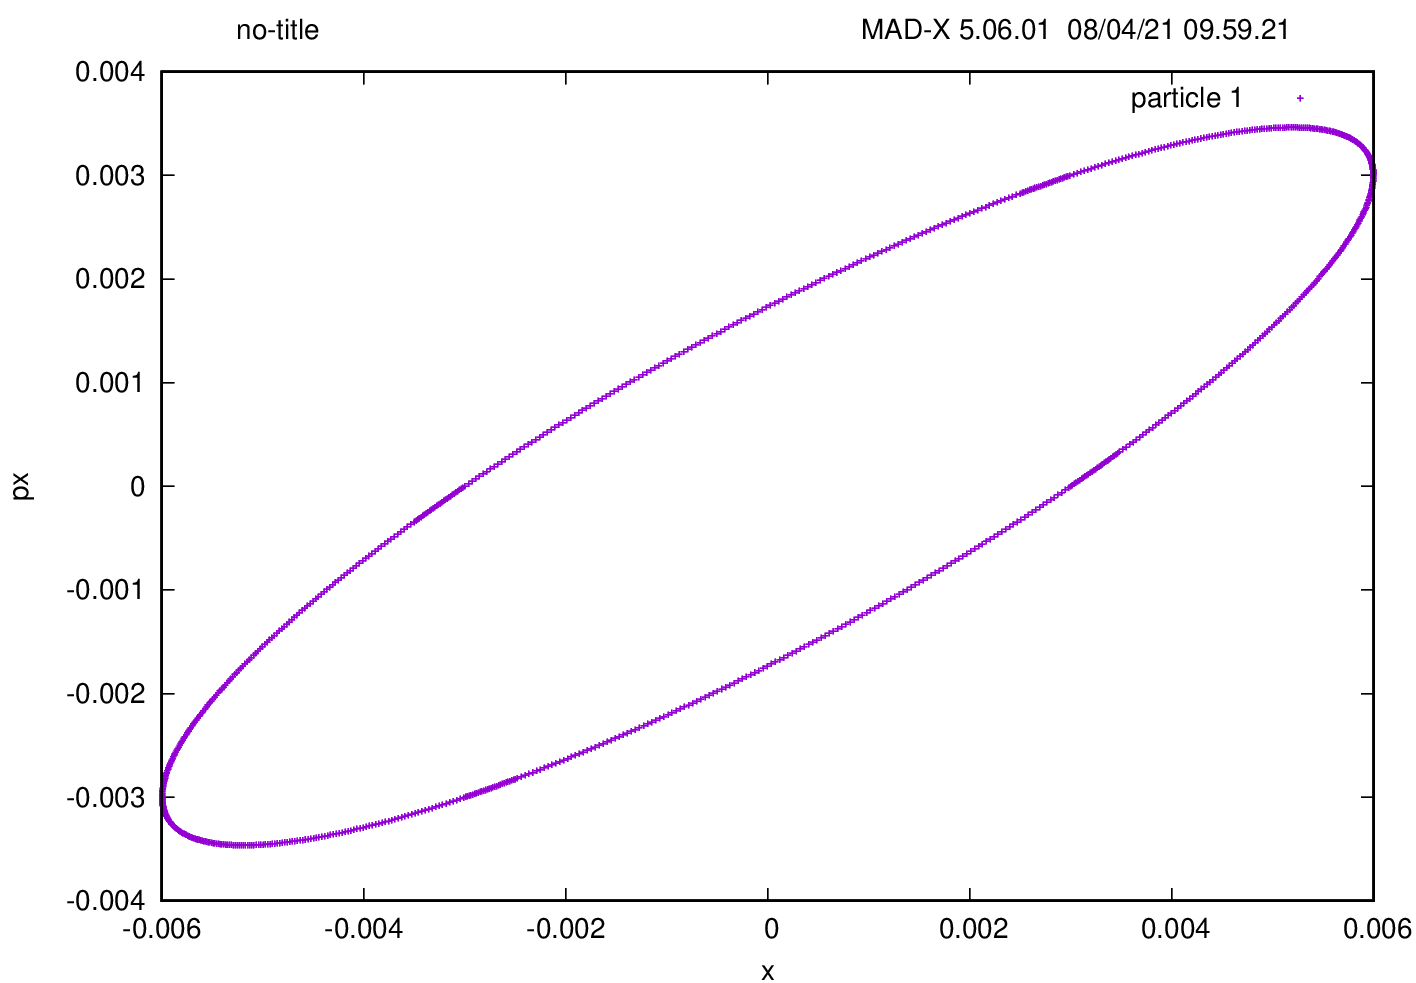
\includegraphics[width=\textwidth]{../../part1/d1f1_x.png}
    \end{minipage}\hfill
    \begin{minipage}{0.49\textwidth}
        \centering
        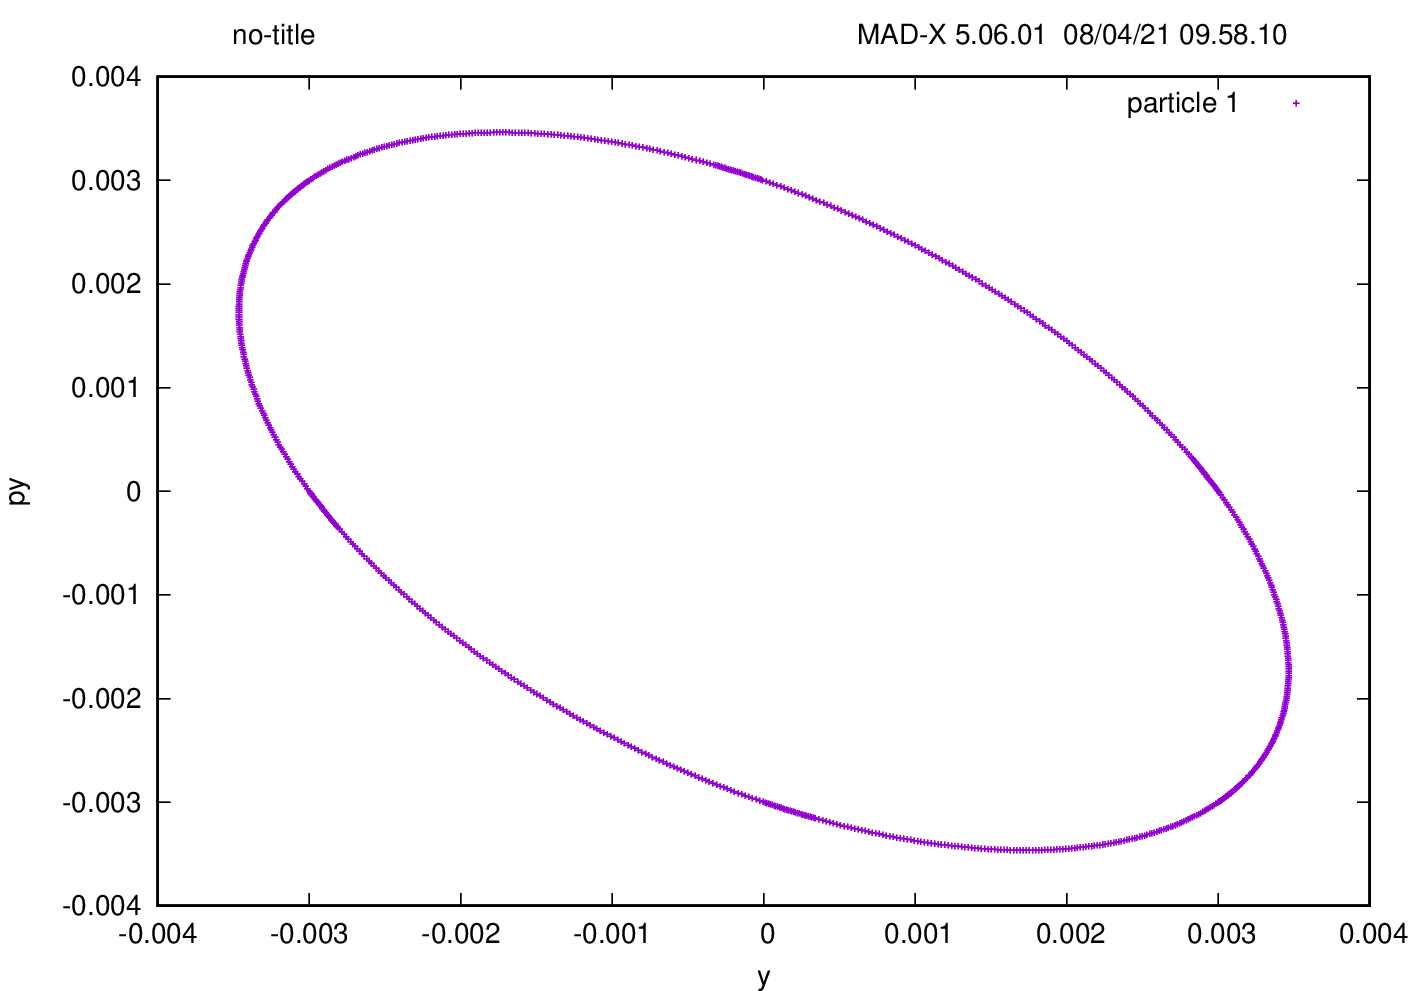
\includegraphics[width=\textwidth]{../../part1/d1f1_y.png}
    \end{minipage}
    \caption{Phase space ellipses for $D=f=1\,\mathrm{m}$}
    \label{fig:ellipse}
\end{figure}

Whether a FODO cell is leading to a stable path can be seen from the stability criterion $|D/(2\cdot f)|<1$.
If this inequality is violated, the particle will be lost as can be seen in figure \ref{fig:unstable}, where $D=2\,\mathrm{m}$ and $f=1\,\mathrm{m}$.

\begin{figure}[tbp]
    \centering
    \begin{minipage}{0.49\textwidth}
        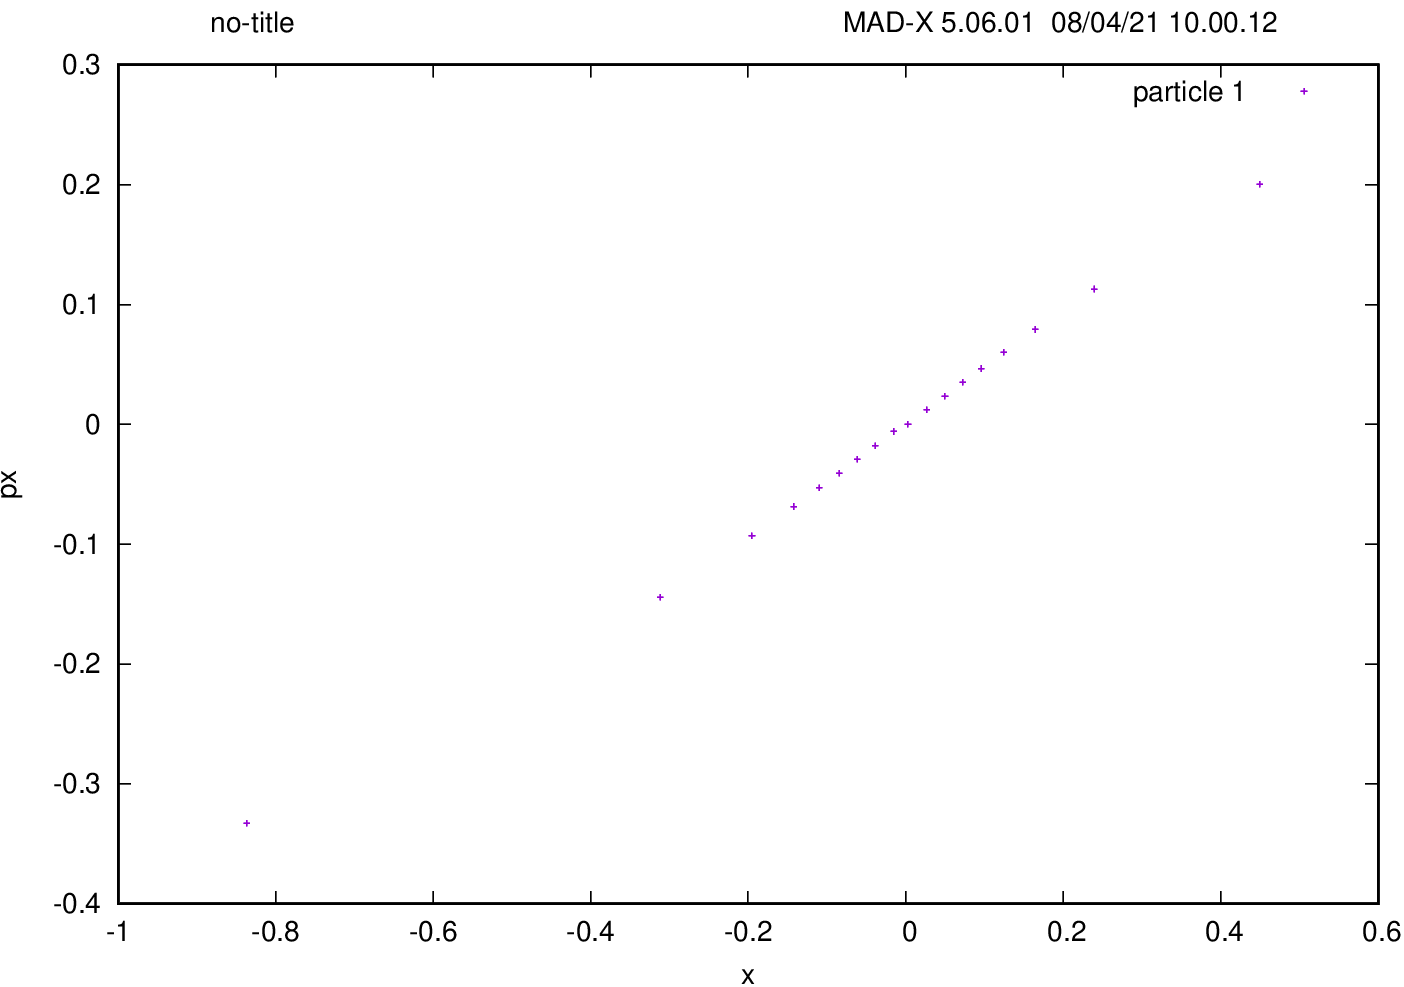
\includegraphics[width=\textwidth]{../../part1/d2f1_x.png}
    \end{minipage}\hfill
    \begin{minipage}{0.49\textwidth}
        \centering
        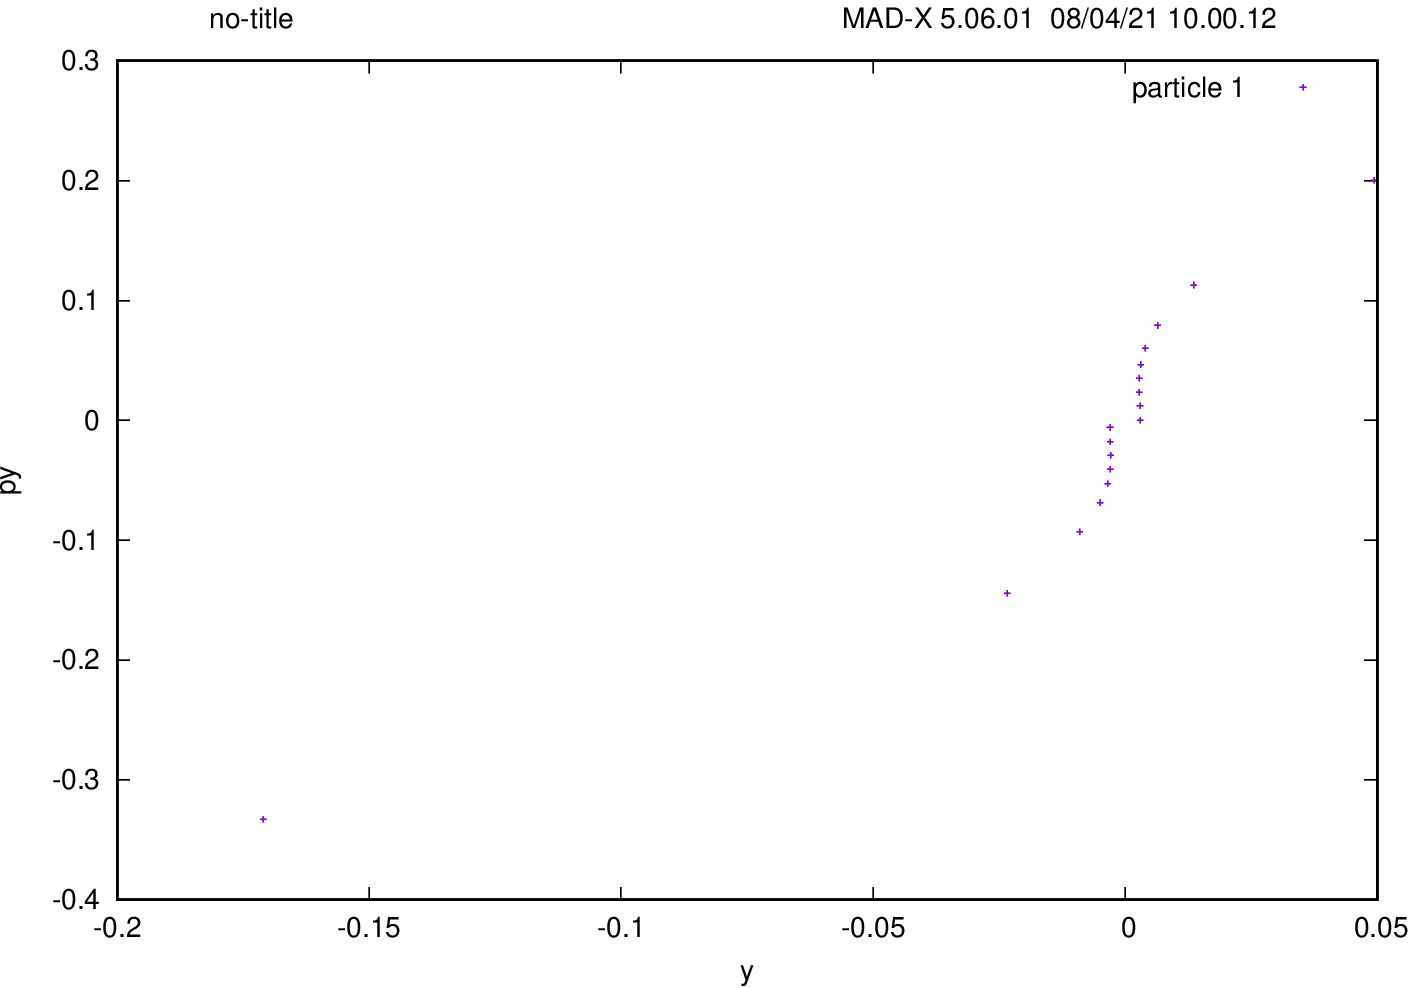
\includegraphics[width=\textwidth]{../../part1/d2f1_y.png}
    \end{minipage}
    \caption{Phase space ellipses for $D=2\,\mathrm{m}, f=1\,\mathrm{m}$}
    \label{fig:unstable}
\end{figure}

One betatron oscillation is complete once the particle did one revolution in phase space. To determine the number of cells necessary to complete one betatron oscillation, the number of turns is reduced until the phase space ellipse is just closed. This is the case for 5 turns, so with the starting point, the ellipse has 6 points (see figure \ref{fig:betatron} exemplary for $y$). As one turn is the pass through one cell, 5 cells are required to complete one betatron oscillation.
\begin{figure}[tbp]
    \centering
    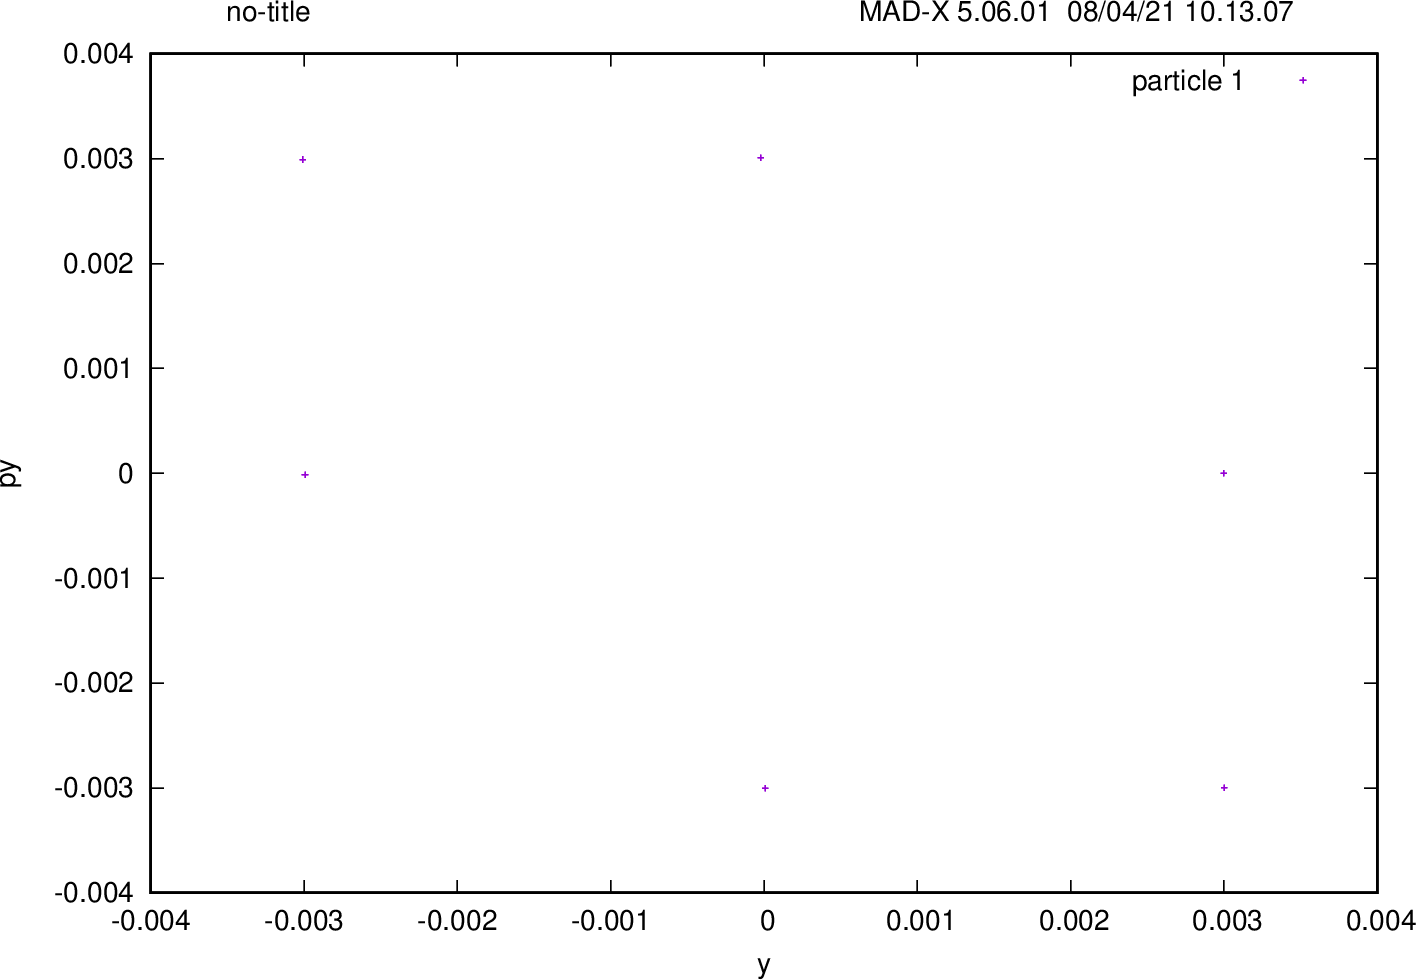
\includegraphics[width=0.55\textwidth]{../../part1/turns5.png}
    \caption{One revolution around the phase space for 5 turns/FODO cells}
    \label{fig:betatron}
\end{figure}

Finally one sextupole is added into the ring before the FODO cell with a stable configuration of $D=1\,\mathrm{m}$, $f=5\,\mathrm{m}$.

\begin{lstlisting}[caption=Defining the FODO cell,label={lst:FODOcell}]
    sx: multipole, knl={0,0,3};

    fodo1: line=(qf, dr, qd,dr);
    ring: line=(sx,fodo1);
\end{lstlisting}

Linear beam elements (as dipoles and quadrupoles) lead to a motion in phase space with the oscillation frequency (phase advance) being independent of the betatron action. The area of the ellipse is a constant of motion for a given starting amplitude. There is no limit on stable amplitudes.\\
Sextupole magnets are nonlinear elements. They are included in beam lines to compensate for chromaticity, i.e. the change in focal length of the quadrupoles with the energy spread of the particles in the beam. They distort the trajectories in phase space more for higher amplitudes and the phase advance is no longer a constant. Islands can appear and the motion becomes increasingly chaotic.

\begin{figure}[tbp]
    \centering
    \begin{minipage}{0.49\textwidth}
        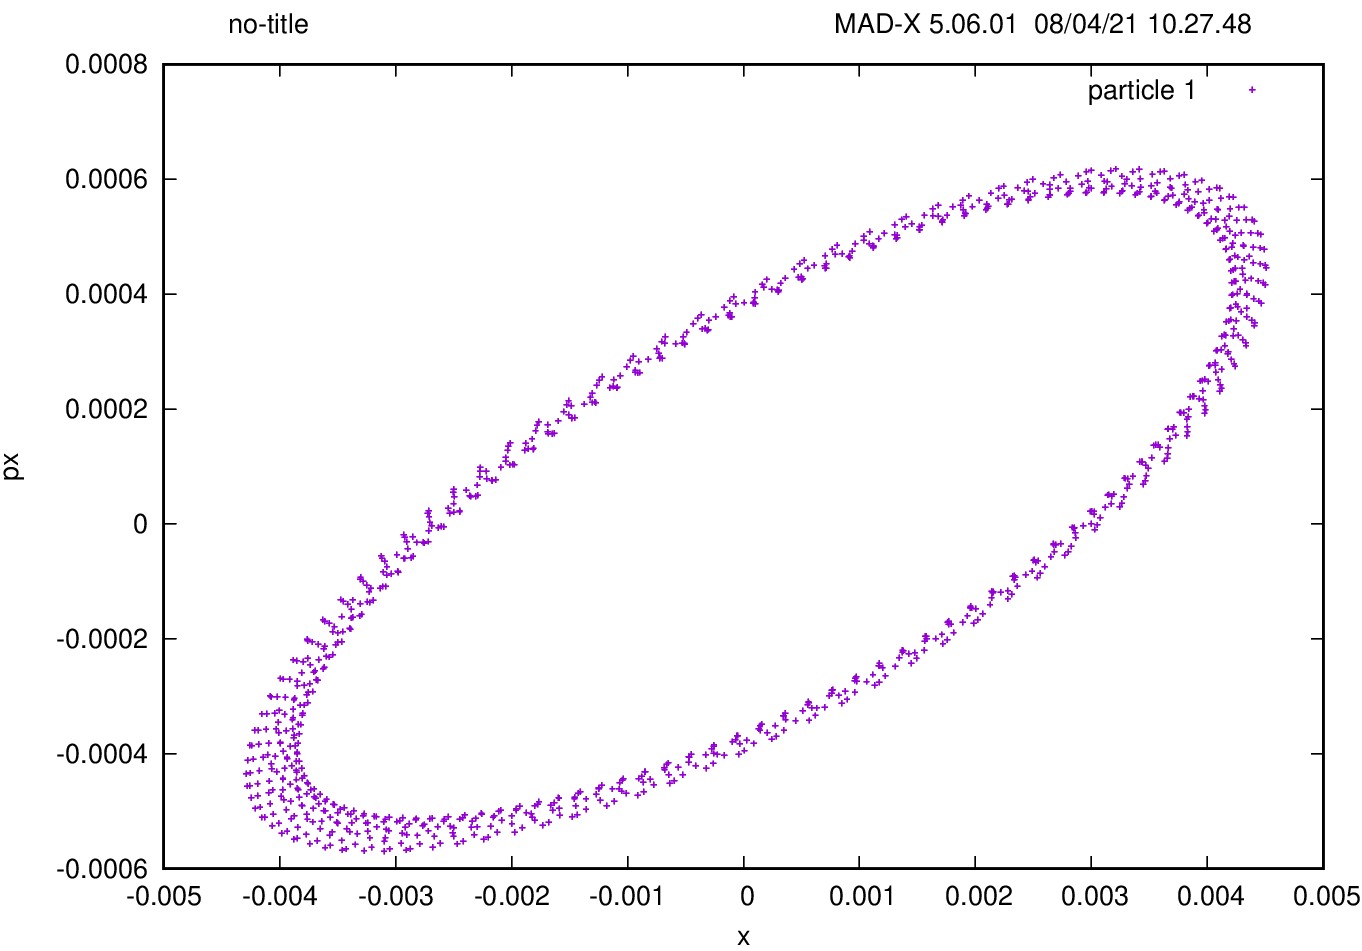
\includegraphics[width=\textwidth]{../../part1/sext1.png}
        \caption{Sextupole strength $1\,\mathrm{T/m^2}$ at $D=1\,\mathrm{m}$, $f=5\,\mathrm{m}$}
        \label{fig:sext1}
    \end{minipage}\hfill
    \begin{minipage}{0.49\textwidth}
        \centering
        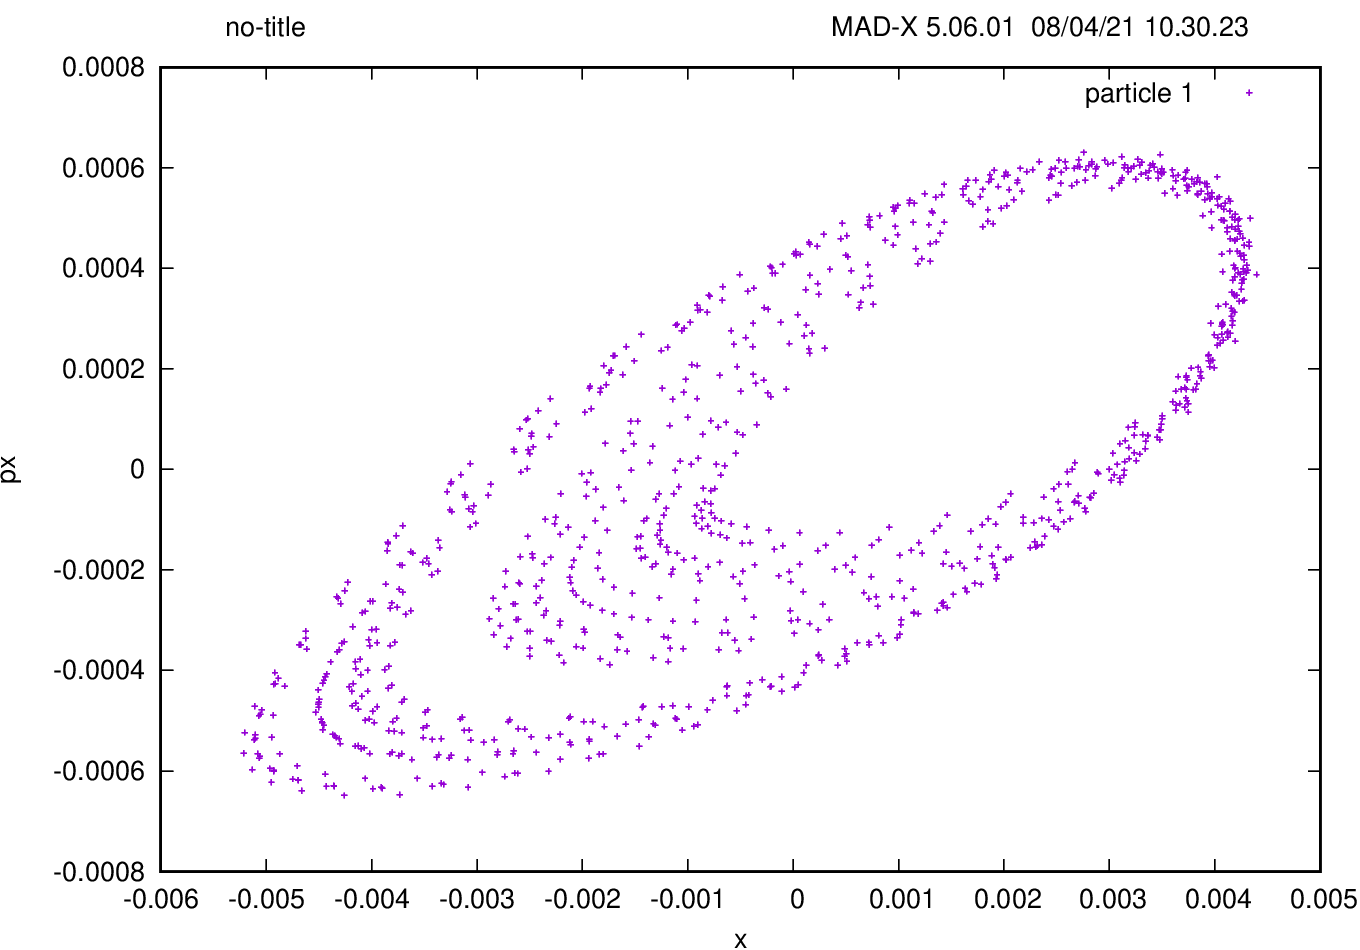
\includegraphics[width=\textwidth]{../../part1/sext4.png}
        \caption{Sextupole strength $4\,\mathrm{T/m^2}$ at $D=1\,\mathrm{m}$, $f=5\,\mathrm{m}$}
        \label{fig:sext4}
    \end{minipage}
\end{figure}

The sextupole's strength is increased from $1\,\mathrm{T/m^2}$ to $4\,\mathrm{T/m^2}$ which results in a more and more disturbed phase space ellipse (see figures \ref{fig:sext1} and \ref{fig:sext4}).
The fun shapes of figures \ref{fig:sext2} and \ref{fig:sext3} were obtained with the combination of $D=f=5\,\mathrm{m}$ and sextupole strengths of $2\text{ and }3\,\mathrm{T/m^2}$.

\begin{figure}[tbp]
    \centering
    \begin{minipage}{0.49\textwidth}
        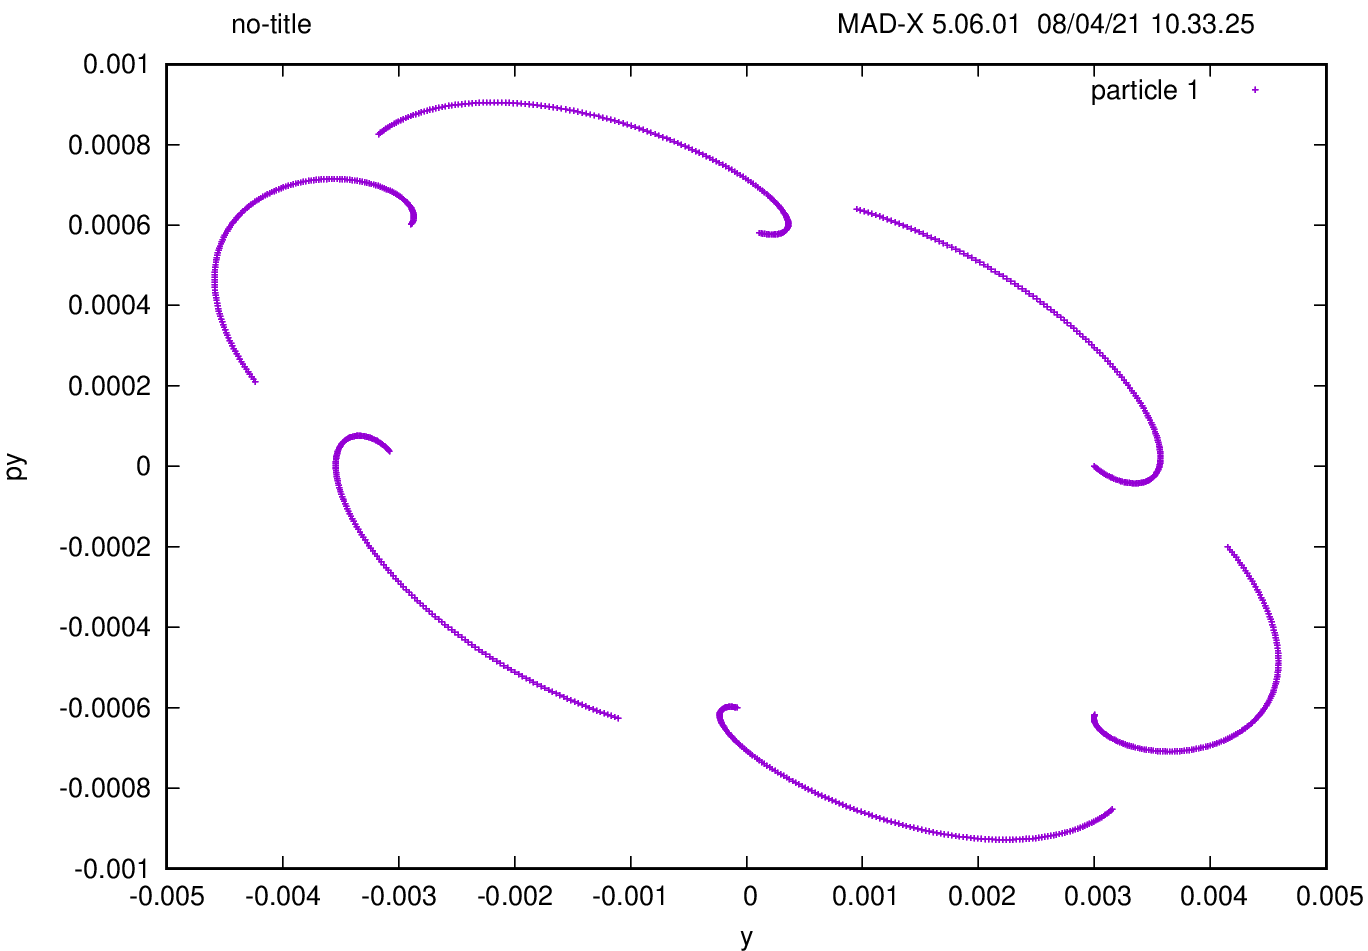
\includegraphics[width=\textwidth]{../../part1/d5f5sx2.png}
        \caption{Sextupole strength $2\,\mathrm{T/m^2}$ at $D=f=5\,\mathrm{m}$}
        \label{fig:sext2}
    \end{minipage}\hfill
    \begin{minipage}{0.49\textwidth}
        \centering
        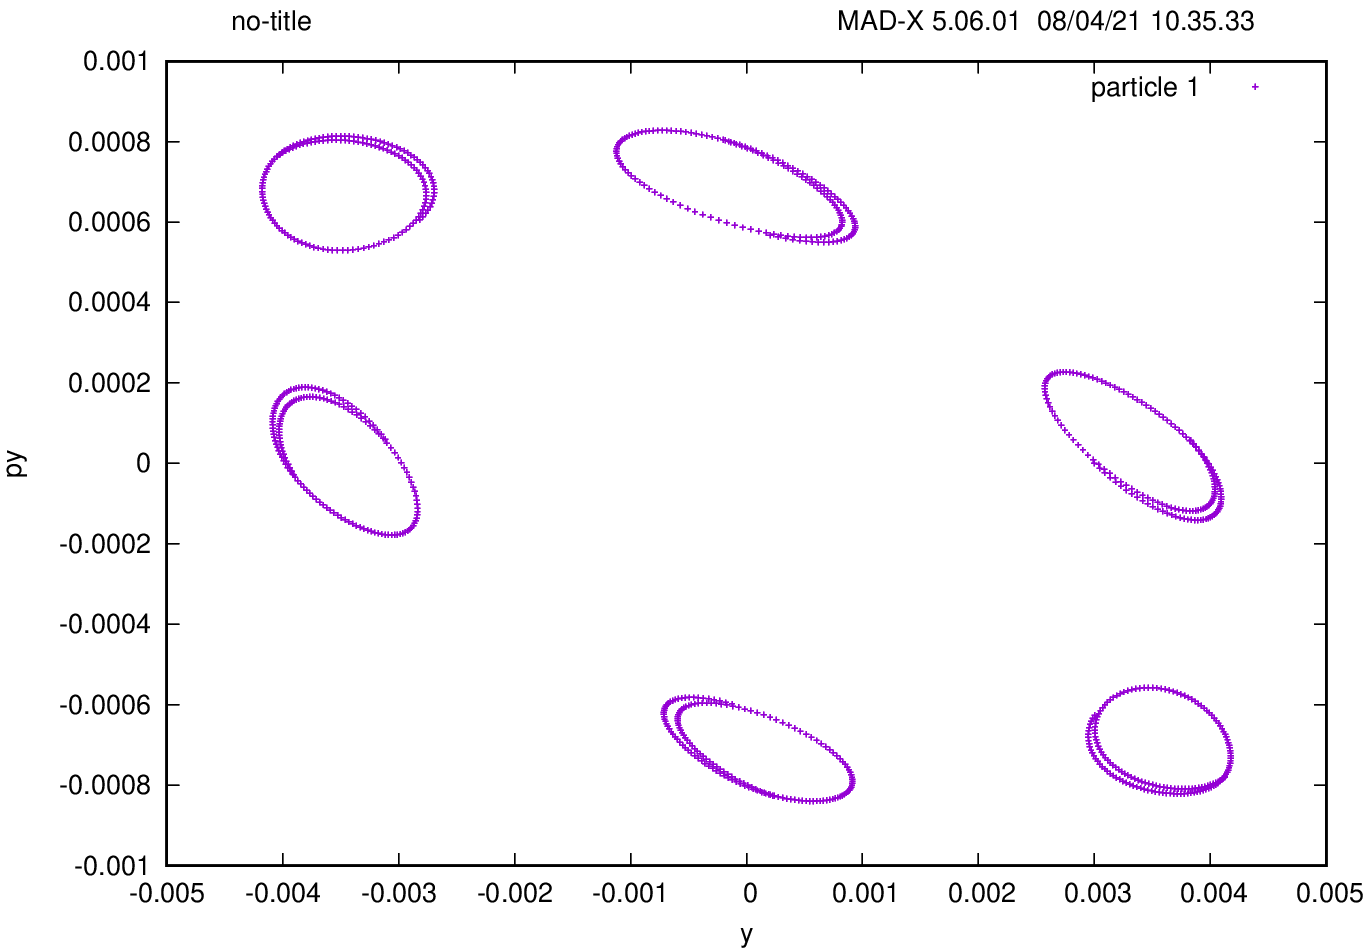
\includegraphics[width=\textwidth]{../../part1/d5f5sx3.png}
        \caption{Sextupole strength $3\,\mathrm{T/m^2}$ at $D=f=5\,\mathrm{m}$}
        \label{fig:sext3}
    \end{minipage}
\end{figure}
\clearpage
\section{Part II - Working with an existing FODO lattice}
In the second part a simplified model of the SPS lattice is studied. The particles are protons at $26\,\mathrm{GeV}$, which currently is the initial energy at injection into the SPS.\\
There are 108 cells in the beam line for one turn. Each of these cells is composed of a focusing quadrupole followed by a focusing sextupole, a drift, two bending magnets, another drift, the defocussing quadrupole and sextupole, a drift, the second pair of dipoles and a final drift. This is illustrated in figure \ref{fig:lattice} and can be seen in the code (listing \ref{lst:sps_lattice}).\\
In the \textit{select} command the parameters to be saved are sest and after with the \textit{twiss} command the calculation of the linear lattice functions and also the chromatic functions is initiated.
\begin{lstlisting}[caption={Definition of SPS lattice}, label={lst:sps_lattice},breaklines=true]
mu=pi/2*0.968;
L=64;
beta_max:=L*(1+sin(mu/2.))/sin(mu);
beta_min:=L*(1-sin(mu/2.))/sin(mu);
alpha_max:=(-1-sin(mu/2.))/cos(mu/2.);
alpha_min:=(1-sin(mu/2.))/cos(mu/2.);
f_max:=L/(4*sin(mu/2.));
f_min:=-L/(4*sin(mu/2.));
D_max:=L*pi/(108.)*(1+0.5*sin(mu/2.))/(4*sin(mu/2)*sin(mu/2))*2;
D_min:=L*pi/(108.)*(1-0.5*sin(mu/2.))/(4*sin(mu/2)*sin(mu/2))*2;
Dpx_max = 0.05660608619;
!value, mu, L, beta_max, beta_min, alpha_max, alpha_min, f_max, f_min, D_max, D_min;
ksf     =                   1.63618409E-02   ;
ksd     =                  -3.35683601E-02   ;

QF: multipole, knl:={0,1./f_max};
QD: multipole, knl:={0,1./f_min};
DD: DRIFT, L:=L/8.;
MBA: SBEND, L:=L/8., ANGLE=pi/108./2;
MBB: SBEND, L:=L/8., ANGLE=pi/108./2;
mm: MARKER;
SF: multipole, knl:={0,0,ksf};
SD: multipole, knl:={0,0,ksd};

FODO: LINE =(QF,SF, DD, MBA,mm,MBB, DD, QD, SD,DD, MBA, mm,MBB, DD);
SPSFODO: LINE =(108*(FODO));

beam,  energy=26, particle=proton;
use, sequence=SPSFODO;
select, flag=twiss,column= name, s, betx, bety, alfx, alfy, dx, mux, muy, angle, k1l, k2l;
select, flag=sectortab, column=name, pos, !k1, k2, k3, k4, k5, k6,
	r11, r12, r13, r14, r15, r16, 
	r21, r22, r23, r24, r25, r26,
	r31, r32, r33, r34, r35, r36,
	r41, r42, r43, r44, r45, r46,
	r51, r52, r53, r54, r55, r56,
	r61, r62, r63, r64, r65, r66;
select, flag=sectormap, range=QF[1]/DD[4];
twiss, deltap=0.00, file=SPS_fodo.twiss, sectormap, sectortable=sectortab, sectorfile=sps_sectormap;
setplot, post=2, lwidth=5,lscale=1.2,rscale=1.5;
PLOT,range=QF[1]/QF[8],HAXIS=s,VAXIS1=betx,bety,vaxis2=dx,colour=100, file=sps_plot;
\end{lstlisting}
\begin{figure}[tbp]
    \centering
    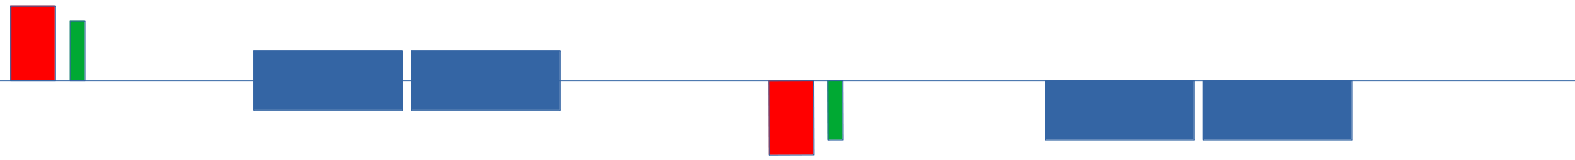
\includegraphics[width=\linewidth]{../../part2/cellSPS.png}
    \caption{Schematic of one cell of the simplified SPS lattice:\\QF-SF–Drift–Dipole A–Dipole B–Drift–QD–SD–Drift–Dipole A–Dipole B–Drift}
    \label{fig:lattice}
\end{figure}

Running the given file with \textit{madx} has three output files. One table (.twiss file extension) where the calculations at the 15 points along the beam line per cell (including the two marker) times 108 cells are saved. The calculated parameters in each point are for example the beta-functions in $x$ and $y$ direction, the dispersion-function, the phase advance and the momentum compaction factors. It also gives the tune and chromaticity, overall momentum compaction factor and maximum and minimum beta and dispersion.\\
The tune in $x$ and $y$ are 
$$q_x=26.1815\text{ and }q_y=26.136$$
and can be found at the beginning of the file. The phase advance per cell is the phase advance at the 15th point, at the end of one cell. Those are $$\mu_x=0.2424\text{ and }\mu_y=0.242\,.$$ The two quantities are related over $$\mu_i=\frac{q_i}{108}\,.$$
\begin{figure}[tbp]
    \centering
    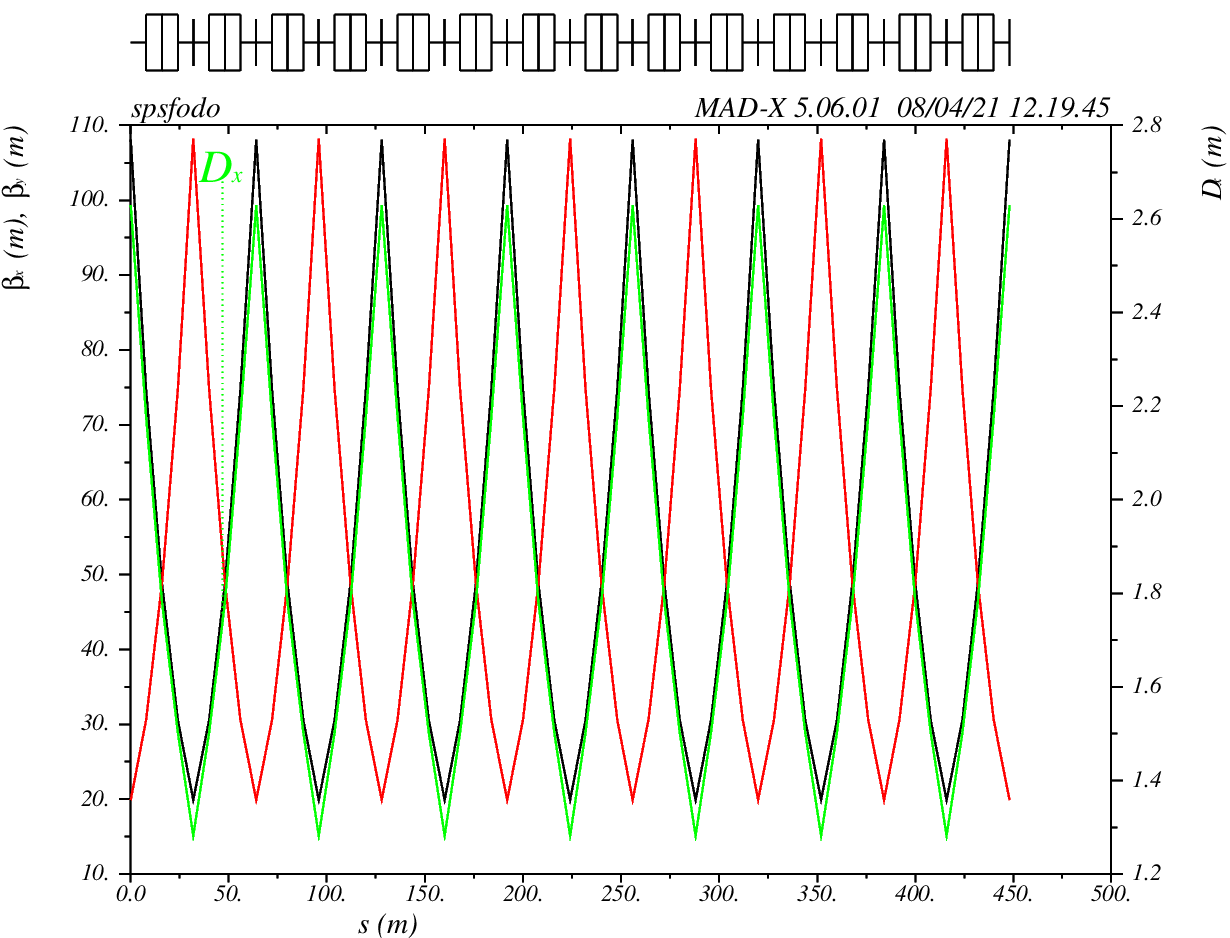
\includegraphics[width=0.8\linewidth]{../../part2/sps_plot.png}
    \caption{Plot of the SPS lattice functions}
    \label{fig:sps_orig}
\end{figure}
\par
The second output are the lattice functions plotted along the beamline as shown in figure \ref{fig:sps_orig} and the third output (sectormap) contains the entries for the transfer matrices of the different elements of the cell.
\par
The quadrupole's strength affect the tune. When increasing the focal length $f_{max}$ and $f_{min}$ both by 50\,\% (times factor 1.5) it leads to the new tunes $$q_x=16.4737\text{ and }q_y=16.40939.$$ The new phase advances per cell are thus $$\mu_x=0.1525\text{ and }\mu_y=0.1519\,.$$\\
But the quadrupoles have no effect on the chromaticity as they are linear field elements, while on the hand a change in the sextupole's strength only affects the chromaticity while not changing the tune.
The original chromaticity is brought almost to zero: $$dq_x=-4.46\cdot 10^{-7}\text{ and }dq_y=-7.207\cdot 10^{-7}.$$ When the strength of both sextupole types, focussing and defocussing, are in raised by 5\,\%, the chromaticity rises to $$dq_x=1.6307\text{ and }dq_y=1.6324\,.$$
\par
The transfer matrix is a $6\times 6$ matrix and is to be multiplied with a vector representing a particle with its position and velocity in $x$ and $y$, its distance $z=-\beta c \Delta t$ with respect to a reference particle and momentum/energy deviation $\delta=\Delta p/p$ also from a reference particle:
\begin{equation}
    \begin{pmatrix}x\\x'\\y\\y'\\z\\\delta\end{pmatrix}_f=\begin{pmatrix}R_{11}&...&&&&\\R_{21}&R_{22}&...&&&\\R_{31}&R_{32}&...&&&\\R_{41}&R_{42}&...&&&\\R_{51}&R_{52}&...&&R_{55}&R_{56}\\R_{61}&R_{62}&...&&R_{65}&R_{66}\end{pmatrix}_{i|f}\cdot \begin{pmatrix}x\\x'\\y\\y'\\z\\\delta\end{pmatrix}_i
\end{equation}
For the SPS the matrix of the last drift space in the cell is
\begin{equation}
    M_{Drift}=\begin{pmatrix}
    1&L_{Drift}&0&0&0&0\\
    0&1&0&0&0&0\\
    0&0&1&L_{Drift}&0&0\\
    0&0&0&1&0&0\\
    0&0&0&0&1&L_{Drift}/\gamma^2\\
    0&0&0&0&0&1
    \end{pmatrix}=
    \begin{pmatrix}
    1&8&0&0&0&0\\
    0&1&0&0&0&0\\
    0&0&1&8&0&0\\
    0&0&0&1&0&0\\
    0&0&0&0&1&0.01043\\
    0&0&0&0&0&1
    \end{pmatrix}\,.
\end{equation}
From this one can read the length of the drift space to be $L_{Drift}=8\,\mathrm{m}$ and the momentum compaction factor to be $\alpha_c=R_{56}=0.01043\,.$
\par
For a thin focusing quadrupole the transfer matrix is
\begin{equation}
    M_{QF}=\begin{pmatrix}
    1&0&0&0&0&0\\
    -1/f_{max}&1&0&0&0&0\\
    0&0&1&0&0&0\\
    0&0&1/f_{max}&1&0&0\\
    0&0&0&0&1&0\\
    0&0&0&0&0&1
    \end{pmatrix}=
    \begin{pmatrix}
    1&0&0&0&0&0\\
    -0.043070&1&0&0&0&0\\
    0&0&1&0&0&0\\
    0&0&0.043070&1&0&0\\
    0&0&0&0&1&0\\
    0&0&0&0&0&1
    \end{pmatrix}\,,
\end{equation}
from which can be concluded that $f_{max}=23.218\,\mathrm{m}=64/\left(4\sin\left(\frac{\pi}{4}0.968\right)\right)\,\mathrm{m}$ which is in agreement with the definition given to \textit{madx}.
Analogously for the thin defocussing quadrupole the matrix is
\begin{equation}
    M_{QD}=\begin{pmatrix}
    1&0&0&0&0&0\\
    -1/f_{min}&1&0&0&0&0\\
    0&0&1&0&0&0\\
    0&0&1/f_{min}&1&0&0\\
    0&0&0&0&1&0\\
    0&0&0&0&0&1
    \end{pmatrix}=
    \begin{pmatrix}
    1&0&0&0&0&0\\
    0.043070&1&0&0&0&0\\
    0&0&1&0&0&0\\
    0&0&-0.043070&1&0&0\\
    0&0&0&0&1&0\\
    0&0&0&0&0&1
    \end{pmatrix}\,,
\end{equation}
and thus $f_{min}=-f_{max}$ as defined.\\
The phase advance per cell in the thin lens approximation is $$\mu=2\arcsin\left(\frac{L_{FODO}}{4f}\right)=2\arcsin\left(\frac{64}{4\cdot 23.218}\right)=1.52055=87^\circ\,,$$
which is very close to the optimal $90^\circ$ for hadrons.
\par
When the sextupoles are switched off the natural chromaticity can be obtained:$$dq_x^{\mathrm{natural}}=-32.6148\text{ and }dq_y^{\mathrm{natural}}=-32.6490\,.$$
These values are very similar in both planes. But to bring the chromaticities close to zero the necessary strength of the in the $x$-plane defocussing sextupole $SD$ is more than double ($ksd=-3.3568\cdot10^{-2}\,\mathrm{T/m^2}$) than the strength of the in the $x$-plane focussing sextupole $SF$ ($ksf=1.6362\cdot10^{-2}\,\mathrm{T/m^2}$).\\
The magnetic field in a sextupole is increases quadratic with the distance from the center.
So particles with a higher dispersion will be deviated more.
As can be seen in figure \ref{fig:sps_orig}, the sextupoles are positioned right after the quadrupoles and the amplitude of dispersion behind the focussing quad $QF$ is higher, i.e. $~2.7\,\mathrm{m}$, than behind the defocussing one $DF$, $~1.3\,\mathrm{m}$, the strength of the focussing sextupoles can be smaller to have the same effect as the defocussing sextupoles.
\par
Finally a sequence of only 8 (instead of 108) FODO cells composing the ring will be investigated.This is achieved by increasing the bending angle per dipole from $\pi/108/2$ to $\pi/8/2$.\\
In figure \ref{fig:sps_mini} the lattice functions for this mini-SPS are shown.
\begin{figure}[tbp]
    \centering
    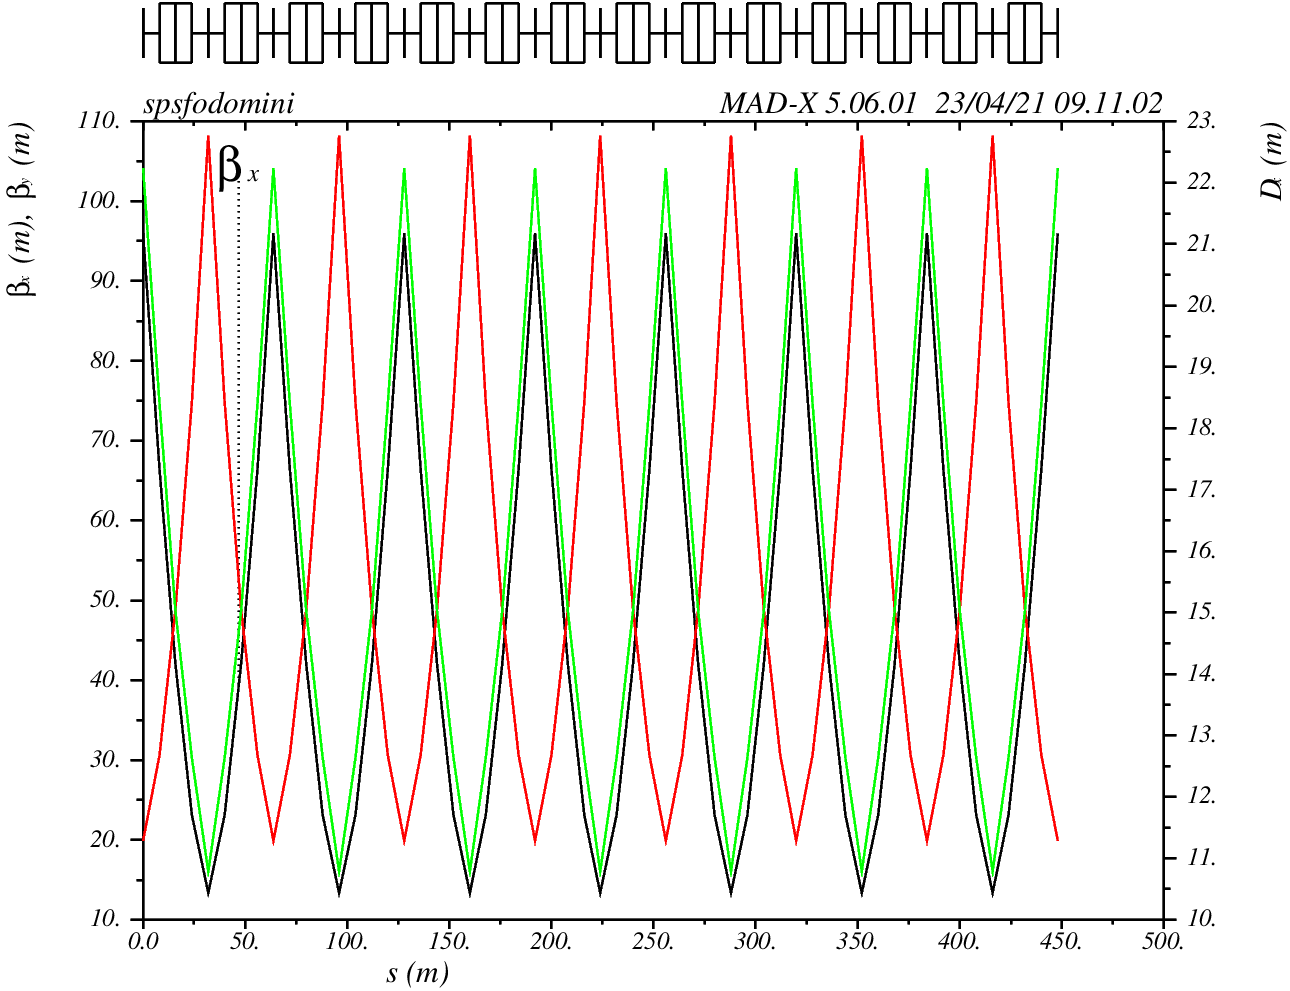
\includegraphics[width=0.8\linewidth]{../../part2/sps_mini.png}
    \caption{Plot of the mini-SPS lattice functions}
    \label{fig:sps_mini}
\end{figure}
As the dipoles are stronger, the dispersion is much higher (about one order of magnitude). And as the weak focussing in the dipoles, which did not have a big effect before, only affects the $x$-plane, with the stronger dipoles the maximum of the beta-function in $x$ is lower than the maximum in $y$-direction.

\clearpage
\section{Part III - Working with the KARA lattice}
This part looks into the real (not an idealised) lattice of KARA.\\
The file \textit{KARA\_lattice.seq} contains the definitions of the different magnet types and families within one type, of the beam position monitors and of the order of the elements to form the overall sequence.
This file is then called in the \textit{madx}-file \textit{run\_kara.madx}, see listing \ref{lst:runKARA}.
\begin{lstlisting}[caption={Run file for the KARA lattice}, label={lst:runKARA},breaklines=true]
// beam parameters
e0 = 2.5;		// beam energy in GeV
mepsx = 42E-9;	// hor. emittance
mepsy = 0.3E-9;	// vert. emittance
mepsl = 0.001;	// long. emittance
mdpp  = 0.001;	// rel. energy spread
msigt = 0.01;	// bunch length

//the sequence definition
CALL, file="KARA_lattice.seq";

//this is the beam  
BEAM, PARTICLE=electron, ENERGY:=e0, EX:=mepsx, EY:=mepsy, radiate;
beam->ET   := mepsl;
beam->SIGE := mdpp;
beam->SIGT := msigt;
// show, beam;

//use this machine
USE, sequence=KARA;

// the RF voltage per cavity in MV
VRFGLOB = 0.35;

// define type and amount out output
select, flag=twiss, clear;
select, flag=twiss, column=name, s, x, betx, bety, dx, dy, alfx, alfy, dpx, dpy;

// calculate the optics
TWISS, deltap=0.0, save,sequence=KARA,file=kara.twiss, chrom;

EMIT, deltap=0.0;
show, beam;

setplot, post=2, lwidth=5,lscale=1.2,rscale=1.5;

// plot closed orbit
PLOT, table=TWISS, HAXIS=s, VAXIS1=x, colour=100, interpolate=false, range=#s/#e, file=kara_plot;

//plot twiss functions and x dispersion
OPTION, -warn;
PLOT,table=TWISS, HAXIS=s, VAXIS1=bety, betx, vaxis2=dx, colour=100, interpolate=true, range=S1.LSS.M/S2.LSS.M;
OPTION, warn;

stop;
\end{lstlisting}

The beam consists of 2.5\,GeV electrons which pass through 4 RF cavities of a voltage of 0.35\,MV each resulting in a total accelerating voltage of 1.4\,MV at a RF frequency of $f_{RF}=500\,\mathrm{MHz}$. The harmonic number is $h=184$.
With the total length of the ring being $L=110.40016\,\mathrm{m}$, the revolution frequency of the electrons is $f_{rev}=2.7155\,\mathrm{MHz}$.
\begin{figure}[tbp]
    \centering
    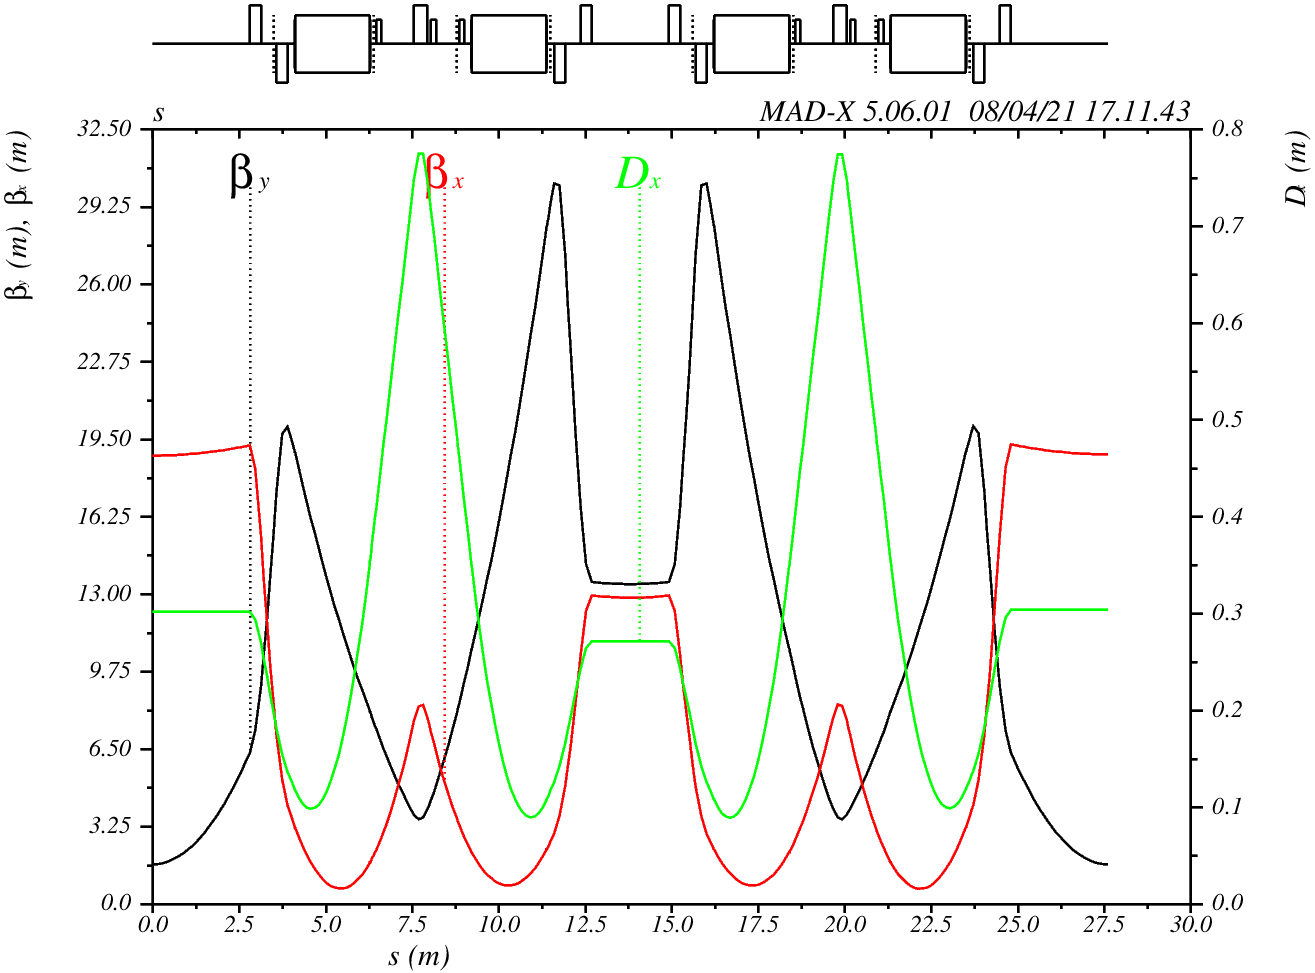
\includegraphics[width=0.8\linewidth]{../../part3/KARA_lattice_orig2.png}
    \caption{Lattice functions of KARA}
    \label{fig:KARAlattice2}
\end{figure}
\begin{figure}[tbp]
    \centering
    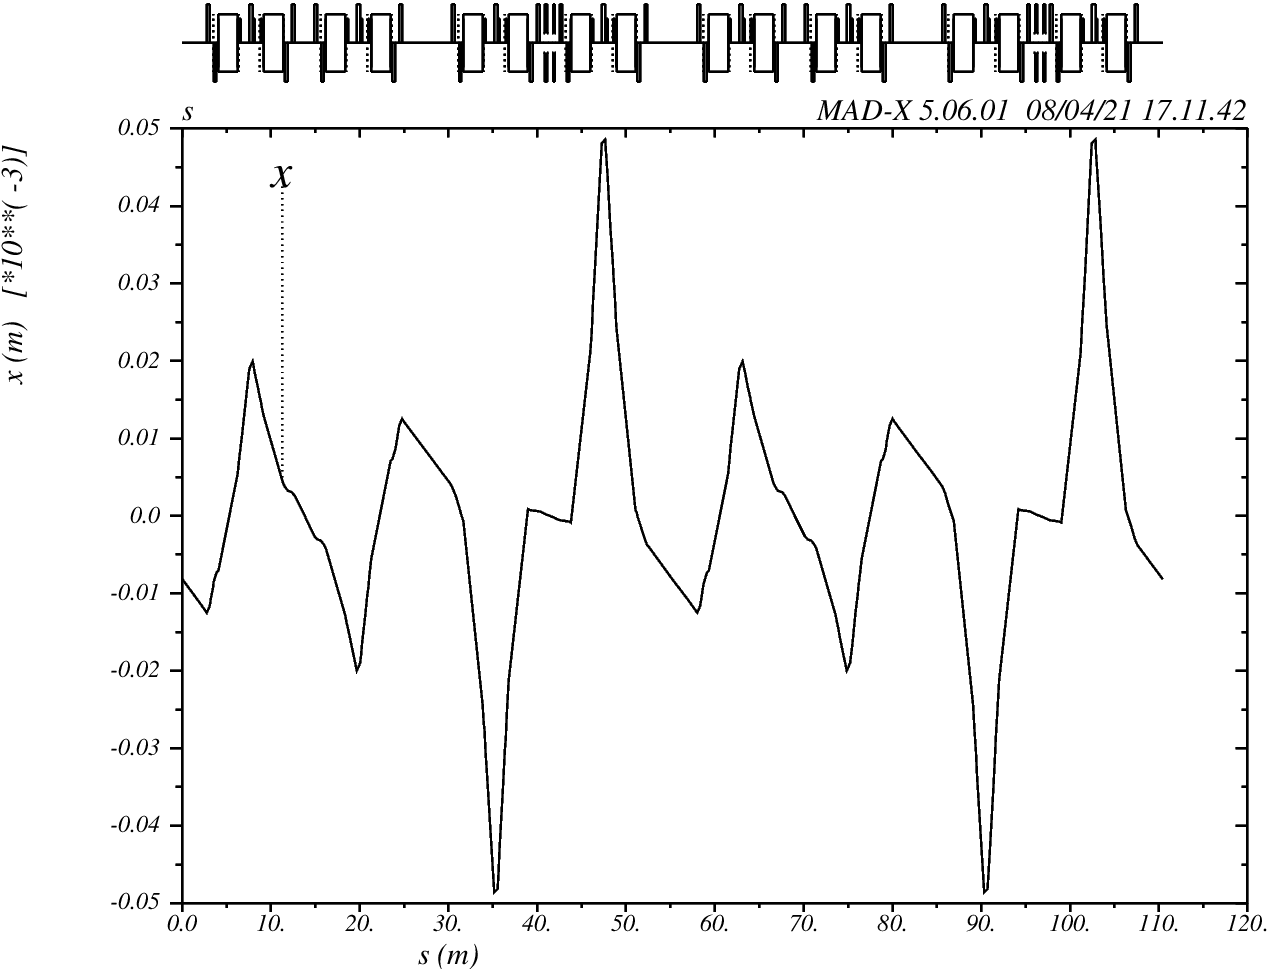
\includegraphics[width=0.8\linewidth]{../../part3/KARA_lattice_orig.png}
    \caption{Closed orbit of KARA}
    \label{fig:KARAlattice}
\end{figure}
\par
Figures \ref{fig:KARAlattice2} and \ref{fig:KARAlattice} show the lattice functions and closed orbit of KARA respectively.
In the output table \textit{kara.twiss} the tunes
$$q_x=6.7947\text{ and }q_y=2.6988$$
and chromaticities
$$dq_x=2.3585\text{ and }dq_y=8.3805$$
can be found.
The momentum compaction factor is $\alpha_c=0.009279$.
\par
When the RF voltage is increased no change in the closed orbit is observed. It is due to the RF cavities merely compensating the synchrotron radiation losses. As long as the losses are fully covered there will be no change in the orbit.
On the other hand when the RF voltage is reduced to $0.15\,\mathrm{MV}$ per cavity the losses are no longer fully compensated and the beam looses energy and eventually hits the inner side of the vacuum chamber, as can be seen in figure \ref{fig:vrf150kV}.
By trying different voltages, the synchrotron radiation losses are determined to lie between $150\,\mathrm{keV}$ and $160\,\mathrm{keV}$.
\begin{figure}[tbp]
    \centering
    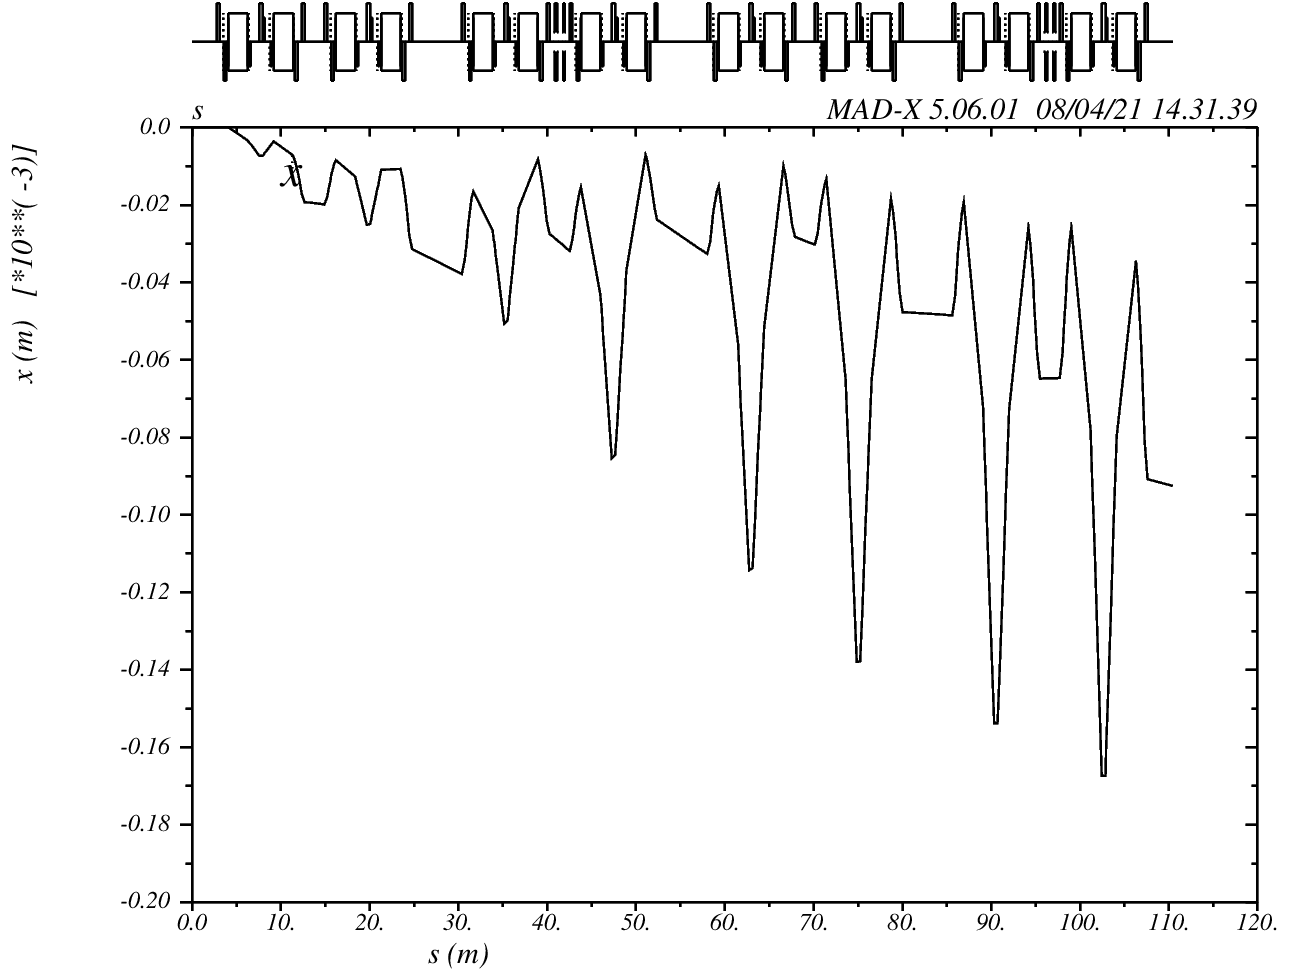
\includegraphics[width=0.8\linewidth]{../../part3/vrf150kV.png}
    \caption{Orbit with $V_{RF}=4\cdot0.15\,\mathrm{MV}$}
    \label{fig:vrf150kV}
\end{figure}
\par
In the following the momentum offset $\Delta p/p$ is varied by $-5\,\%$ to $5\,\%$ and the change in the orbit at two BPM's in the first sector and in tune and chromaticity are noted down, see table \ref{tab:3c}.
\begin{table}[tbp]
    \centering
    \small
    \begin{tabular}{r|r r r r r r}
dp&x bpm1&x bpm2&q1&q2&dq1&dq2\\\hline
-0.005&-0.00114271&-0.00180591&6.78833&2.66069&0.303642&6.91681\\
-0.002&-0.000431372&-0.000748750&6.79090&2.68270&1.4478&7.76801\\
0&-9.19809e-06&6.69311e-06&6.79468& 2.69884&2.35845&8.38054\\
0.002&0.000363002&0.000807854&6.80044&2.71626&3.4301&9.04647\\
0.005&0.000805192&0.00210926&6.81363&2.74507&5.47128&10.1974
    \end{tabular}
    \caption{Change in orbit and tune with momentum offset}
    \label{tab:3c}
\end{table}
Plotting the $x$-position over $\Delta p/p$ the dispersion can be obtained as the gradient of the linear fit in figure \ref{fig:3cDispersion}.
The dispersion at the first BPM is $$D_{x1}=0.19531\,\mathrm{m}$$ while the \textit{madx} calculation with no momentum offset from before yielded $$D_{x1}^{dp=0}=0.19918\,\mathrm{m}.$$ Same procedure for the second BPM gives a dispersion of $$D_{x2}=0.39119\,\mathrm{m}$$ while the calculation from before gave $$D_{x2}^{dp=0}=0.38916\,\mathrm{m}.$$ Both value are in good agreement considering that only 5 data points were used for the fit.
\begin{figure}[tbp]
    \centering
    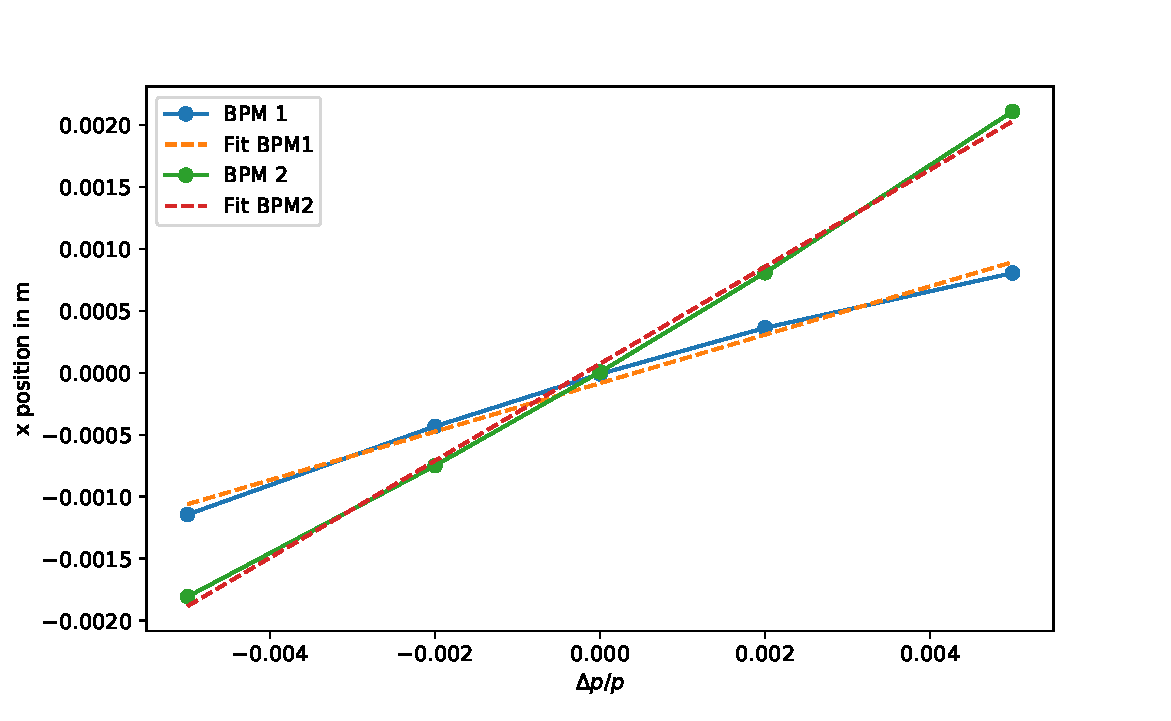
\includegraphics[width=0.8\linewidth]{../../part3/3c_dispersion.pdf}
    \caption{$x$-position over momentum offset}
    \label{fig:3cDispersion}
\end{figure}
\par
Plotting the fractional tunes $q_x$ and $q_y$ over $\Delta p/p$ a quadratic fit can be made from which the linear term gives the chromaticities in the 2 directions, see figures \ref{fig:3cChroma1} and \ref{fig:3cChroma2}.
The values from the fits are $$dq_x=2.51030\text{ and }dq_y=8.43099$$ compared to the values calculated by \textit{madx} before $$dq_x^{dp=0}=2.51030\text{ and }dq_y^{dp=0}=8.43099.$$
\begin{figure}[tbp]
\begin{minipage}{0.49\textwidth}
        \centering
        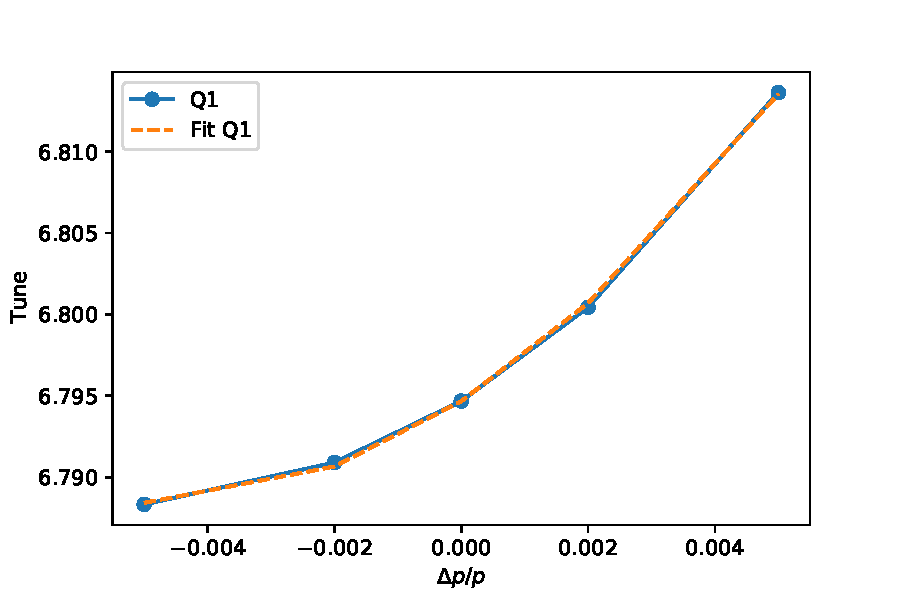
\includegraphics[width=1.1\linewidth]{../../part3/3c_chroma.pdf}
        \caption{Fractional tune in $x$ over momentum offset}
        \label{fig:3cChroma1}
    \end{minipage}\hfill
    \begin{minipage}{0.49\textwidth}
        \centering
        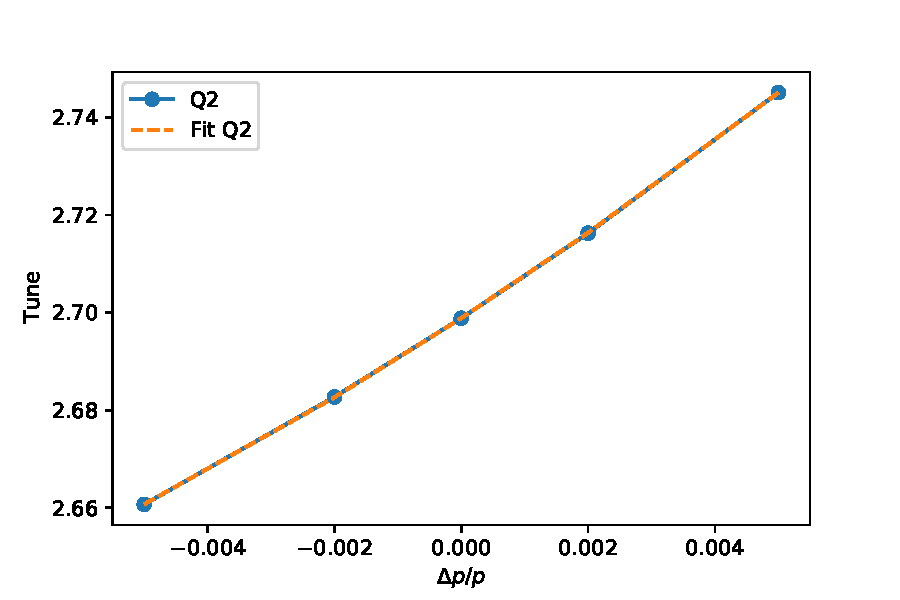
\includegraphics[width=1.1\linewidth]{../../part3/3c_chroma2.pdf}
        \caption{Fractional tune in $y$ over momentum offset}
        \label{fig:3cChroma2}
    \end{minipage}
\end{figure}
\par
\begin{table}[tbp]
    \centering
    \small
    \begin{tabular}{r|r r r}
quad family&percent of kq&q1& q2\\\hline
1& 0.95&6.229655577& 2.82254419\\
1&1.05&7.147677581&2.522960645\\
2& 0.95&6.902549973&2.229925233\\
2&1.05&6.660147605&3.180405389\\
3&0.95&6.601481415&2.766610311\\
3&1.05&6.979753402&2.533548305\\
4&0.98&6.817540159&2.348782014\\
4&1.05&6.711702721&3.155251723\\
5&0.95&6.496700785&2.937224266\\
5&1.05&7.033816694&2.223021106
    \end{tabular}
    \caption{Change in fractional tunes with strength of the different quadrupole families}
    \label{tab:3d}
\end{table}
In order to verify the gradient error formula
$$\delta Q=\frac{1}{4\pi}\,\beta_0\,\Delta k\,l$$
the strength of one quadrupole family at a time is slightly changed ($\pm5\,\%$) and the change in tune is noted, see table \ref{tab:3d}.\\
The original values for the tunes and beta-functions without any change in the quadrupole strength are:
\begin{itemize}
    \item $q_x=6.794679$
    \item $q_y=2.698843$
    \item ${\beta_0}_{x,\;family1,\;quad1}=15.51\,\mathrm{m}$
    \item ${\beta_0}_{x,\;family1,\;quad2}=19.24\,\mathrm{m}$
    \item ${\beta_0}_{y,\;family1,\;quad1}=9.144\,\mathrm{m}$
    \item $l_{quad,\;family3}=0.39\,\mathrm{m}$
    \item $l_{quad,\;default}=0.32\,\mathrm{m}$
\end{itemize}
So for $\Delta k=+5\,\%$ in the first quadrupole family, the change in tune is $\delta Q_x=0.353$.
Compared to the calculation with the above equation, with the factor of $\frac{1}{4}$ as there are 4 pairs of the quadrupoles of family one, gives:
$$\delta Q_x=\frac{1}{4\cdot4\pi}({\beta_0}_{x,\;family1,\;quad1}+{\beta_0}_{x,\;family1,\;quad2})\cdot 2.1152 \cdot0.05\cdot l_{quad,\;default}=0.37435\,.$$
\par
If not a whole family is strengthened by $5\,\%$ but only one single quadrupole, the new fractional tunes are $$q_x^{single}=6.8414\text{ and }q_y^{single}=2.6425\,.$$
So the change in tune is $$\delta Q_x=0.0467\text{ and }\delta Q_y=0.05633\,.$$
Comparing this to the calculation
$$\delta Q_x=\frac{1}{4\pi}{\beta_0}_{x,\;family1,\;quad1}\cdot 2.1152 \cdot0.05\cdot l_{quad,\;default}=0.04177\;\text{and}$$
$$\delta Q_y=\frac{1}{4\pi}{\beta_0}_{y,\;family1,\;quad1}\cdot 2.1152 \cdot0.05\cdot l_{quad,\;default}=0.02463\,.$$
it can be seen that the $x$-direction agrees rather well while the $y$=direction's change in tune is about double than calculated.
\par
The last part will look at the natural chromaticity of KARA.
In the case of accelerating electrons a chromaticity of about 1 is wanted for better stability. As chromaticity leads to tune spread it can help to stabilise certain parts of the accelerator.\\
On the other hand, if the chromaticity is too big parts of the bunch could have a tune which hits resonances and thus leads to instabilities. So some chromaticity is wanted but it has to be controlled and not exceed certain levels.\\
When all sextupoles are switched off, the natural chromaticity are
$$dq_{x\;\mathrm{natural}}=-13.347\text{ and }dq_{y\;\mathrm{natural}}=-6.8974\,.$$
With all sextupoles at nominal strength the chromaticities become:
$$dq_{x}=2.358\text{ and }dq_{y}=8.381\,.$$